\documentclass[a4paper]{article}
\usepackage{a4wide,amssymb,epsfig,latexsym,multicol,array,hhline,fancyhdr}
\usepackage{amsmath}
\usepackage{lastpage}
\usepackage[lined,boxed,commentsnumbered]{algorithm2e}
\usepackage{enumerate}
\usepackage{color}
\usepackage{graphicx}	\usepackage{chemformula}		
\usepackage{indentfirst}
% Standard graphics package
\usepackage{amsmath}
\usepackage{siunitx}
\usepackage{textcomp}
\usepackage{array}
\usepackage{tabularx, caption}
\usepackage{multirow}
\usepackage{multicol}
\usepackage{rotating}
\usepackage{graphics}
\usepackage{geometry}
\usepackage{setspace}
\usepackage{epsfig}
\usepackage{tikz}
\usetikzlibrary{arrows,snakes,backgrounds}
\usepackage{hyperref}
\usepackage{booktabs}
\hypersetup{urlcolor=blue,linkcolor=black,citecolor=black,colorlinks=true} 
%\usepackage{pstcol} 								% PSTricks with the standard color package

\newtheorem{theorem}{{\bf Theorem}}
\newtheorem{property}{{\bf Property}}
\newtheorem{proposition}{{\bf Proposition}}
\newtheorem{corollary}[proposition]{{\bf Corollary}}
\newtheorem{lemma}[proposition]{{\bf Lemma}}

\AtBeginDocument{\renewcommand*\contentsname{Contents}}
\AtBeginDocument{\renewcommand*\refname{References}}
%\usepackage{fancyhdr}
\setlength{\headheight}{40pt}
\pagestyle{fancy}
\fancyhead{} % clear all header fields
\fancyhead[L]{
 \begin{tabular}{rl}
    \begin{picture}(25,15)(0,0)
    \put(0,-8){
\includegraphics[width=8mm, height=8mm]{Image/hcmut.png}}
    %\put(0,-8){\epsfig{width=10mm,figure=hcmut.eps}}
   \end{picture}&
	%
\includegraphics[width=8mm, height=8mm]{hcmut.png} & %
	\begin{tabular}{l}
		\textbf{\bf \ttfamily University of Technology, Ho Chi Minh City}\\
		\textbf{\bf \ttfamily Faculty of Computer Science and Engineering}
	\end{tabular} 	
 \end{tabular}
}
\fancyhead[R]{
	\begin{tabular}{l}
		\tiny \bf \\
		\tiny \bf 
	\end{tabular}  }
\fancyfoot{} % clear all footer fields
\fancyfoot[L]{\scriptsize \ttfamily Assignment for Mathematical Modelding - Academic year 2020 - 2021}
\fancyfoot[R]{\scriptsize \ttfamily Page {\thepage}/\pageref{LastPage}}
\renewcommand{\headrulewidth}{0.3pt}
\renewcommand{\footrulewidth}{0.3pt}


%%%
\setcounter{secnumdepth}{4}
\setcounter{tocdepth}{3}
\makeatletter
\newcounter {subsubsubsection}[subsubsection]
\renewcommand\thesubsubsubsection{\thesubsubsection .\@alph\c@subsubsubsection}
\newcommand\subsubsubsection{\@startsection{subsubsubsection}{4}{\z@}%
                                     {-3.25ex\@plus -1ex \@minus -.2ex}%
                                     {1.5ex \@plus .2ex}%
                                     {\normalfont\normalsize\bfseries}}
\newcommand*\l@subsubsubsection{\@dottedtocline{3}{10.0em}{4.1em}}
\newcommand*{\subsubsubsectionmark}[1]{}
\makeatother


\begin{document}

\begin{titlepage}
\begin{center}
VIETNAM NATIONAL UNIVERSITY, HO CHI MINH CITY \\
UNIVERSITY OF TECHNOLOGY \\
FACULTY OF COMPUTER SCIENCE AND ENGINEERING
\end{center}

\vspace{1cm}

\begin{figure}[h!]
\begin{center}

\includegraphics[width=3cm]{Image/hcmut.png}
\end{center}
\end{figure}

\vspace{1cm}


\begin{center}
\begin{tabular}{c}
\multicolumn{1}{l}{\textbf{{\Large MATHEMATICAL MODELING (CO2011)}}}\\
~~\\
\hline
\\
\multicolumn{1}{l}{\textbf{{\Large Assignment}}}\\
\\
\textbf{{\Huge Dynamical systems in forecasting}}\\
\\
\textbf{{\Huge Greenhouse Micro-climate}}\\
\\
\hline
\end{tabular}
\end{center}

\vspace{3cm}

\begin{table}[h]
\begin{tabular}{rrl}
\hspace{5 cm} & Advisor: & Nguyen Tien Thinh\\
& Students: & Ngo Tu Duy - 1752133 (CC01) \\
& & Truong Van Quang Dat - 1652142 (CC03) \\
& & Quach Dang Giang - 1952044 (CC02) \\
& & Hoang Tran Viet Long - 1652350 (CC01)\\
& & Nguyen Dinh Tuan - 1552411 (CC02)\\
\end{tabular}
\end{table}

\begin{center}
{\footnotesize HO CHI MINH CITY, DECEMBER 2020}
\end{center}
\end{titlepage}


%\thispagestyle{empty}

\newpage
\tableofcontents
\newpage


%%%%%%%%%%%%%%%%%%%%%%%%%%%%%%%%%
\section{Member list \& Workload}
\begin{center}
\begin{tabular}{|c|c|c|l|c|}
\hline
\textbf{No.} & \textbf{Fullname} & \textbf{Student ID} & \textbf{Problems} & \textbf{Percentage of work}\\
\hline 
%%%%%Student 1%%%%%%%%%%
\multirow{3}{*}{1} & \multirow{3}{*}{Ngo Tu Duy} & \multirow{3}{*}{1752133} & $50\%$ 4  &
\multirow{3}{*}{$20$ \%}\\
 & &  & $50\%$ 5 &\\
 & &  &  &\\
\hline 
%%%%%Student 2%%%%%%%%%%%
\multirow{3}{*}{2} & \multirow{3}{*}{Truong Van Quang Dat} & \multirow{3}{*}{1652142} & $10\%$ 2 &
\multirow{3}{*}{$20\%$ }\\
 & &  & $50\%$ 5 &\\
 & &  &   &\\
 %& &  & $?$ 3 &\\
\hline
%%%%%Student 3%%%%%%%%%%%
\multirow{3}{*}{3} & \multirow{3}{*}{Quach Dang Giang (Leader)} & \multirow{3}{*}{1952044} & $70\%$ 1 &
\multirow{3}{*}{$20$ \%}\\
 & &  & $30\%$ 2 &\\
 & &  & $40\%$ 3 &\\
\hline
%%%%%Student 4%%%%%%%%%%%
\multirow{3}{*}{4} & \multirow{3}{*}{Hoang Tran Viet Long} & \multirow{3}{*}{1652350} & $20\%$ 1 &
\multirow{3}{*}{$20$ \%}\\
 & &  & $50\%$ 2 &\\
 & &  & $60\%$ 3 &\\
\hline
%%%%%Student 5%%%%%%%%%%%
\multirow{3}{*}{5} & \multirow{3}{*}{Nguyen Dinh Tuan} & \multirow{3}{*}{1552411} & $10\%$ 1 &
\multirow{3}{*}{$20$ \%}\\
 & &  & $10\%$ 2 &\\
 & &  & $50\%$ 4 &\\
\hline
\end{tabular}
\end{center}


%%%%%%%%%%%%%%%%%%%%%%%%%%%%%%%%%
\section{Exercise 1}
	\subsection{Problem 1a}
	
	\bigskip
 Dynamical systems are mathematical objects used to model physical phenomena whose state (or instantaneous description) changes over time. These models are used in financial and economic forecasting, environmental modeling, medical diagnosis, industrial equipment diagnosis, and a host of other applications.
    To study dynamical systems mathematically, we represent them in terms of differential equations.
    
    The state of dynamical system at an instant of time is described by a point in an n-dimensional space called the \textbf{state space} (the dimension n depends on how complicated the systems is) . As time passes the point moves, sweeping out a curve in the state space, called a \textbf{trajectory} of the system (mathematically, this curve is a solution of the governing differential equations)
   
    A system can be classified according to different criteria, such as
    
    \bigskip
\begin{table}[h]
\centering
\begin{tabular}{|c|c|}
\hline
\multicolumn{2}{|c|}{System Classification}     \\ \hline
\textit{\textbf{Either}} & \textit{\textbf{Or}} \\ \hline
Deterministic            & Stochastic           \\ \hline
Discrete                 & Continous            \\ \hline
Linear                   & Nonlinear            \\ \hline
Autonomous               & Nonautomonous        \\ \hline
\end{tabular}%

\end{table}
\bigskip
\bigskip
    
A deterministic system has an entirely predictable behavior. The system is fully understood, and it is possible to predict exactly what will happen. A stochastic model, on the other hand, possess inherent randomness that make it impossible to predict its behavior. 

A discrete system changes the state variables only at a countable number of points in time. Dynamical systems with discrete time, like the ideal coin toss, have their states evaluated only after certain discrete intervals. In the case of the coin toss, the smooth tumbling and bouncing of the coin is ignored, and its state is only viewed when it has come to equilibrium. These points in time are the ones at which the event occurs/change in state. A continuous system, however, change in a continuous way, and not abruptly from one state to another, ex: A pendulum swinging back and forth,...

In a linear system, function describing the system behavior must satisfied 2 basic properties:

\[Addictivity: f(x+y)=f(x)+f(y)\]
\[Homogeneity: f(\alpha x) = \alpha f(x)\]

A nonliner system's function simply doesn't satisfied the above requirements.

An autonomous system is a system of ordinary differential equations, which do not depend on the independent variable. If the independent variable is time, we call it time-invariant system.

A nonautonomous system is a system that doesn't satisfied the above requirements.

In this assignment, we use the dynamical system especially the first order differential equation to predict the changes of CO2 inside a greenhouse model


\subsection{Problem 1b}
The first order differential equations in the dynamical system with the initial value $y_0$ and $t_0$ can be re-written as:
\[
\left\{\begin{array}{ll}
\frac{dy}{dx} & =f(x, y) \\
y\left(x_{0}\right) & =y_{0}
\end{array}\right.
\]

Suppose we have a linear differential equation 
\[y+p(x)y=g(x)\] in which p and g are continous functions on the open interval I = $(\alpha,\beta)$. Then for each $t \in I$ there exists a unique solution $y=\phi(t)$ to the differential
equation $\frac{dy}{dx}+p(x)y=g(x)$  that also satisfies the initial value condition $y(x_0)=y_0$
\subsection{Problem 1c}

A differential equation is an equation which contains one or more terms and the derivatives of one variable (i.e., dependent variable) with respect to the other variable (i.e., independent variable). The order of the equation is equal to the highest order of the derivative in the equation, therefore a first-order differential equation only have first-order derivative in their equation

\[\frac{dy}{dx} = f(x)\]

We often have to find a particular solution which specifies the value of the unknown function at a given point in the domain. This is called an initial-value problem.
For example, solve the diferential equation:

\[\Dot{y} = 2(25-y)\] Knowing that
\[y(0) = 40\]

We can see that if y(t) = 25 then it will satisfy the first equation but y(0) = 25 $\neq$ 40. So y(t) = 8 is not a solution. So as long as y is not 8, we can rewrite the equation as

\[\frac{dy}{dt}\frac{1}{25-y} = 2 \]
\[\Leftrightarrow \frac{1}{25-y}dy =2dt\]
\[\Leftrightarrow  \int \frac{1}{25-y} dy = \int 2dt\]
\[\Leftrightarrow ln\lvert 25 - y\rvert * (-1) = 2t + C_0\]
\[\Leftrightarrow ln\lvert 25 - y\rvert = -2t - C_0 = -2t + C\]
\[\Leftrightarrow \lvert 25 - y\rvert = e^{-2t+C}\]
\[\Leftrightarrow y - 25 = \pm  e^C e^{-2t}\]
\[\Leftrightarrow y = 25 \pm e^C e^{-2t} = 25 + Ae^{-2t}\]

A is some non-zero constant. Since we want y(0) = 40, we substitute and solve for A:
\[40 = 25 + Ae^0\]
\[A = 15\]
Thus $y = 25 + 15e^{-2t}$ is the solution of the differential equation.

\subsection{Problem 1d}
\begin{itemize}
    \item Explicit Euler
\end{itemize}
In mathematics and computational science, the Euler method (also called forward Euler method) is a first-order numerical procedure for solving ordinary differential equations (ODEs) with a given initial value. It is the most basic explicit method for numerical integration of ordinary differential equations and is the simplest Runge–Kutta method. 

Explicit methods calculate the state of the system at a later time from the state of the system at the current time without the need to solve algebraic equations. For the method, we begin by choosing a step size or $\Delta t$. The size of $\Delta t$ determines the accuracy of the approximate solutions as well as the number of computations. Graphically this method produces a series of line segments, which thereby approximates the solution curve. 

Given $\frac{dy}{dt}=f(t,y)$ with $y(t_0)=y_0$ we approximate the path of the solution by:

\begin{enumerate}
    \item Step size:  First, we choose the step size $h$ which is the size of the increments along the t-axis that we will use in approximation. Smaller increments tend to give more accurate answers, but then there are more steps to compute. 
    \item Compute slope: Compute the slope $\frac{dy}{dt} = f(t_0,y_0)$
    \item Get next point: The next point is $t_1 = t_0 + h$ and $y_1 = y_0 + f(t_0,y_0)h$
    \item Repeat: : Repeat the last two steps with $(t_1,y_1)$
\end{enumerate}
\begin{figure}[h]
    \centering
    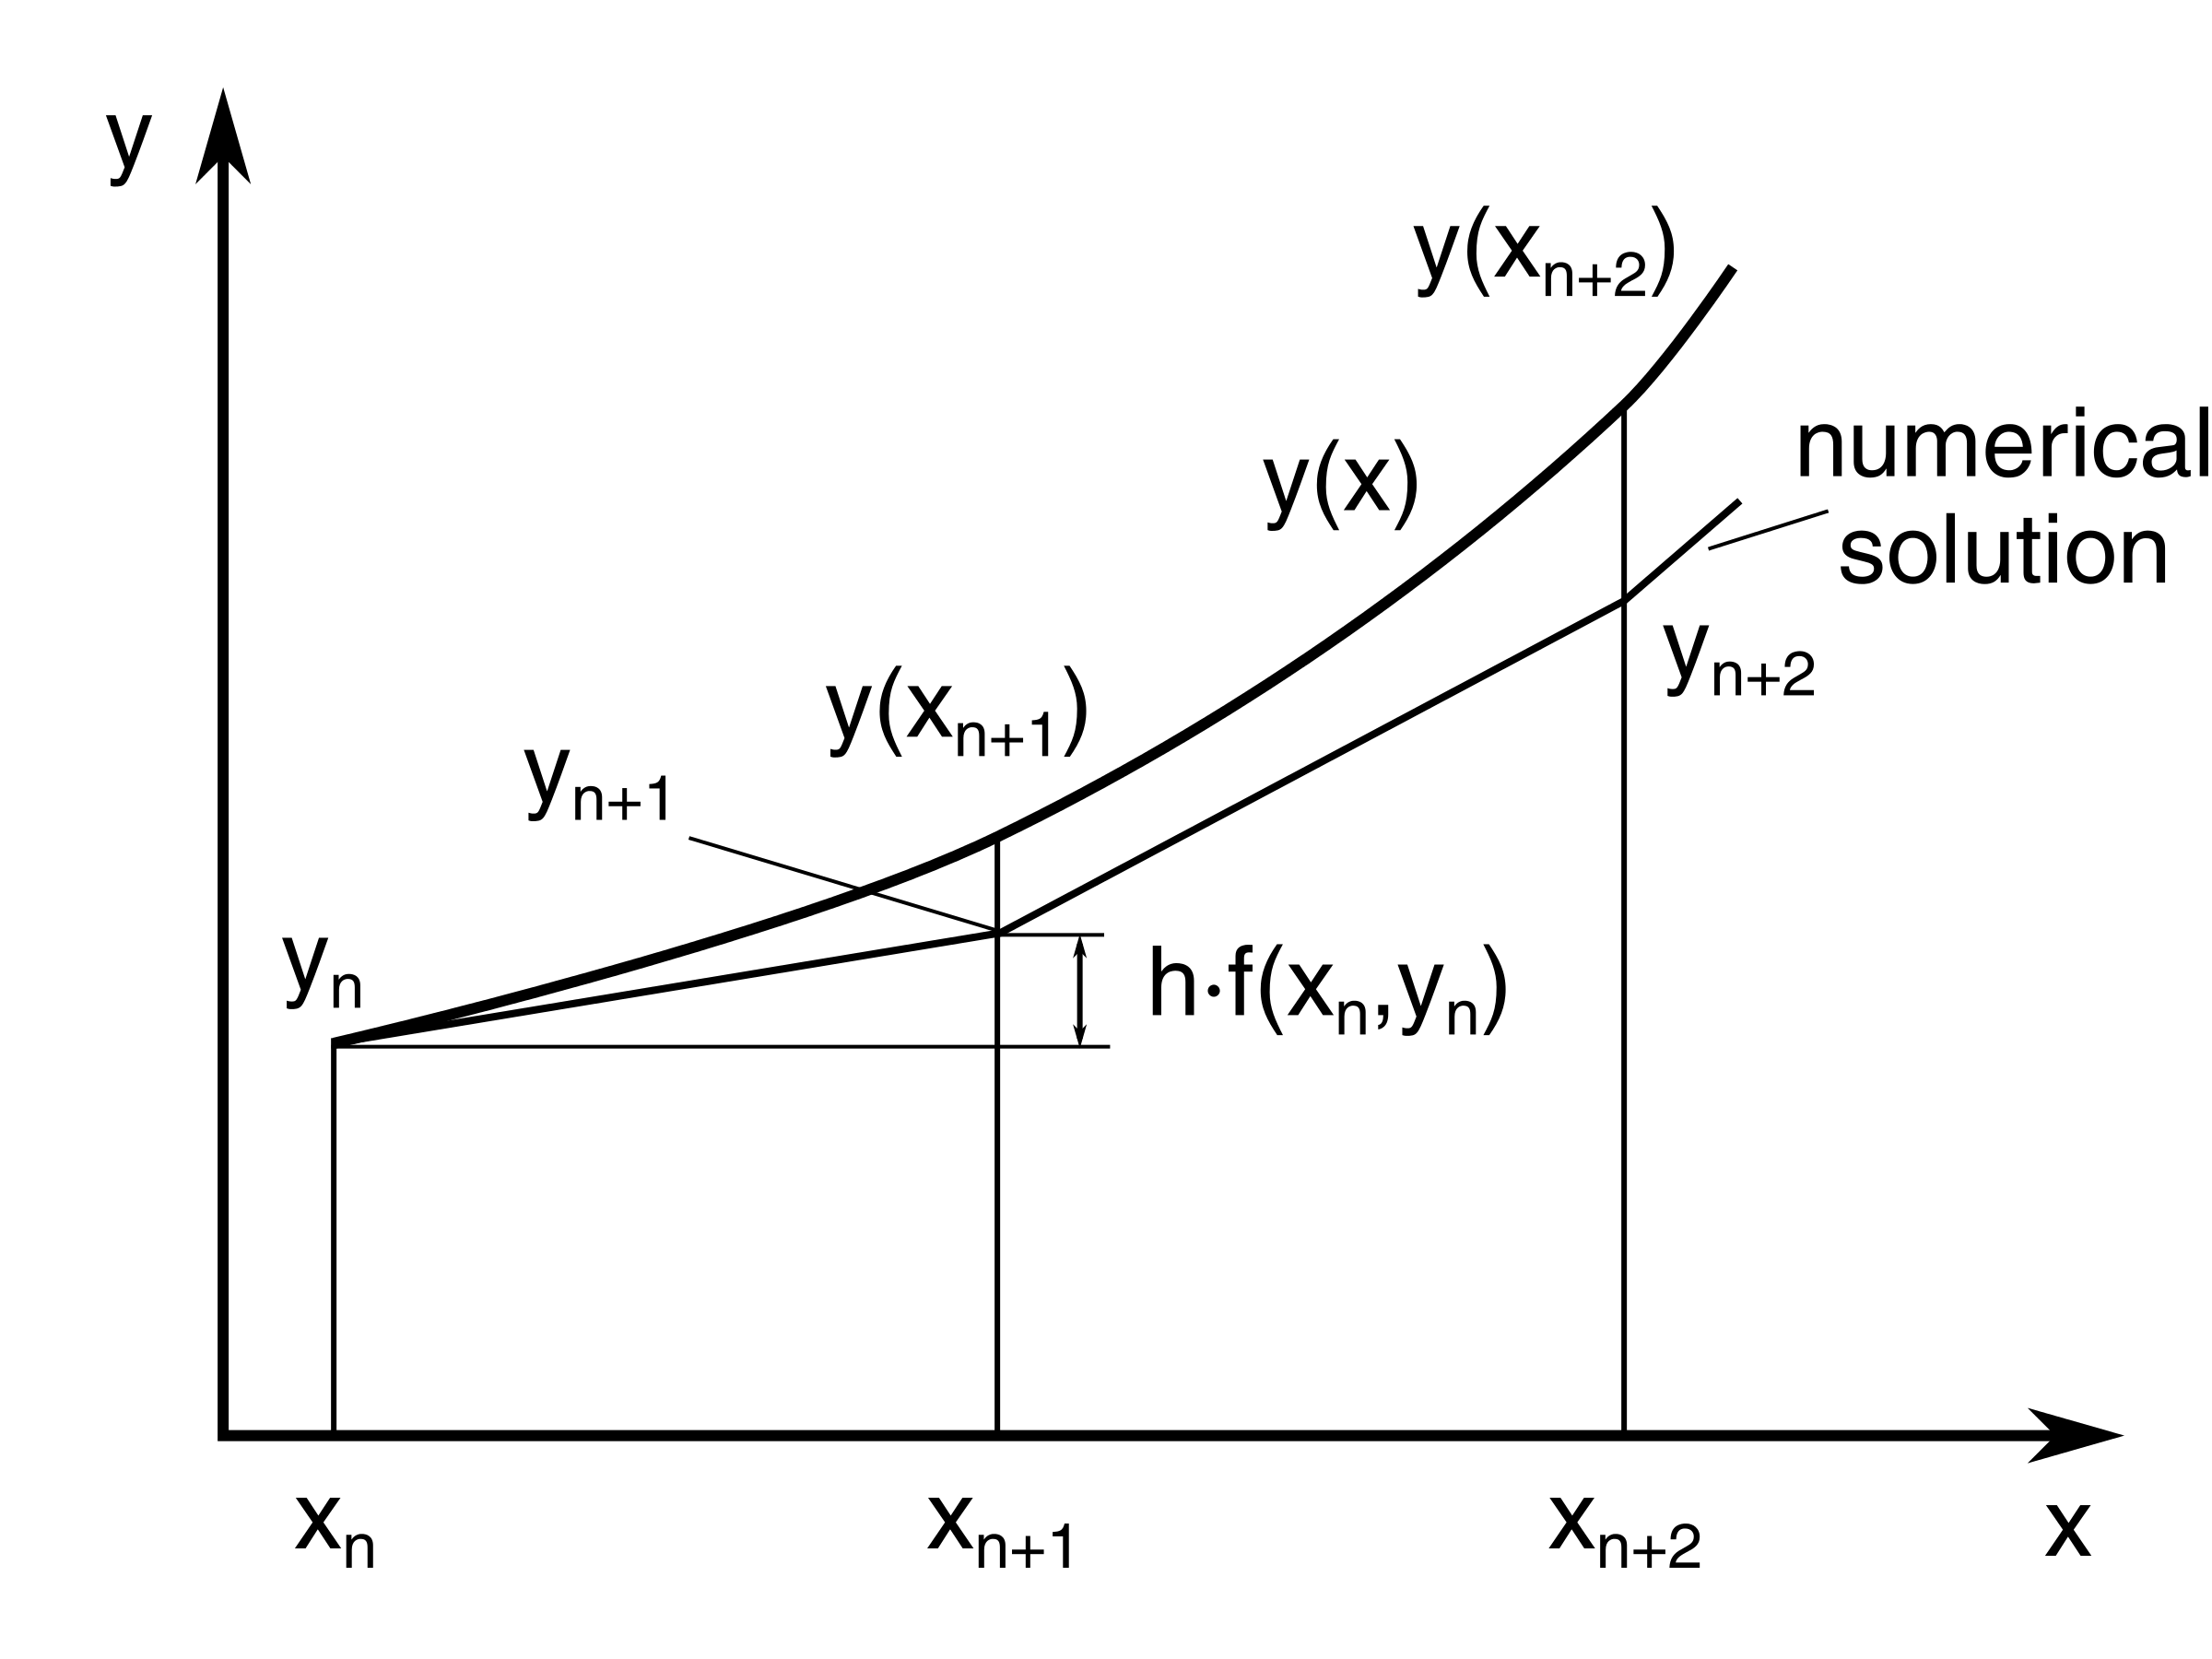
\includegraphics[width = 2in, height = 2in]{Code/Pic/Euler.png}
    \caption{Explicit Euler metho}
    \label{fig:my_label}
\end{figure}
\begin{itemize}
    \item Explicit Runge–Kutta of order 4
\end{itemize}
In numerical analysis, the Runge–Kutta methods are a family of implicit and explicit iterative methods, which include the well-known routine called the Euler Method, used in temporal discretization for the approximate solutions of ordinary differential equations. The most widely known member of the Runge–Kutta family is generally referred to as "RK4", the "classic Runge–Kutta method" or simply as "the Runge–Kutta method".

Supoose we have a problem: $\frac{dy}{dt}=f(t,y)$ with $y(t_0)=y_0$
With y is an unknown function (scalar or vector) of time $t$,  which we would like to approximate. We also know the rate of change $\frac{dy}{dt}$ is a function of y and t; and the initial value.
 First,  we choose the step sizehwhich is the size of the increments along thet-axis that we will use in approximation. We define
 \[y_{n+1}=y_n+\frac{1}{6}h(k_1+2k_2+3k_3+4k_4\]
 \[t_{n+1}=t_n+h\]
 for n = 0,1,2,3,..... with
 \[k_1=f(t_n,y_n)\]
 \[k_2=f(t_n+\frac{h}{2},y_n+h\frac{k_1}{2})\]
 \[k_3=f(t_n+\frac{h}{2},y_n+h\frac{k_2}{2})\]
 \[k_4=f(t_n+h,y_n+h k_3)\]
 Here, by using the RK4 approximation, we get the next value $y_{n+1}$ using present value $y_n$ and the weighted average of four increments, where each increment is the product of the size of the interval, h  and an estimated slope specified by function f on the right-hand side of the differential equation.
 
$k_1$  is the slope at the beginning of the interval, using y (Euler's method).

$k_2$ is the slope at the midpoint of the interval, using $y$ and $ k_1$.

$k_3$ is also the slope at the midpoint, but now using $y$ and $k_2$.

$k_4$ is the slope at the end of the interval, using $y$ and $k_3$

\noindent    In averaging the four slopes, greater weight is given to the slopes at the midpoint. 
\subsection{Problem 1e}  

Given that,
\[\Dot{y} = 2(25-y)\] and
\[y(0) = 40\]

Find y(0.1)

We know the solution is $y = 25 + 15e^{-2t}$. We choose h = 0.1

\textbf{Euler method}: 
\begin{align*}
   y(0.1) &= y_0+hf(y_0,t_0)\\
        &= 40+0.1(2(25-40))\\
        &= 37
\end{align*}

\textbf{RK4 method}:
\[k_1=2(25-40)=-30\]
\[k_2=2(25-38.5)=-27\]
\[k_3=2(25-38.65)=-27.3\]
\[k_4=2(25-37.2)=-24.54\]


$y(0.1) = y(0)+\frac{1}{6}h(k_1+2k_2+3k_3+4k_4)=36.599$



True y(0.1) = $25+15e^{-2*0.1} \approx 37.28 $



%%%%%%%%%%%%%%%%%%%%%%%%%%%%%%%%%
\section{Exercise 2}
\subsection{Problem 2a}

\begin{figure}[h]
    \centering
    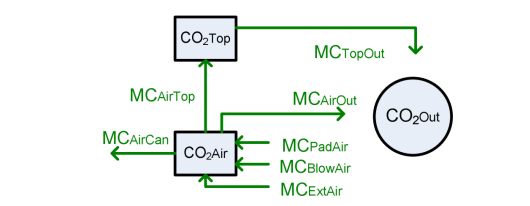
\includegraphics[width = 5in, height = 2in]{Code/Pic/figure.PNG}
    \caption{The $CO_2$ flow inside and outside a greenhouse}
    \label{fig:my_label}
\end{figure}

\begin{figure}[h]
    \centering
    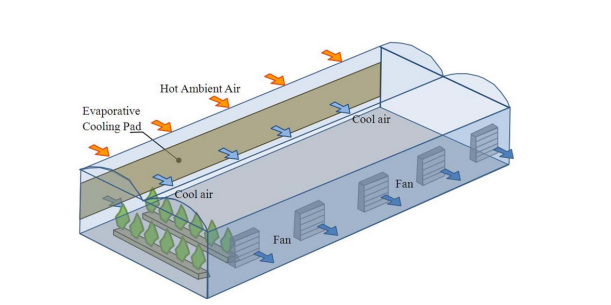
\includegraphics[width = 5in, height = 2in]{Code/Pic/green.png}
    \caption{The movement of $CO_2$ through the pad system and fan system.}
    \label{fig:my_label}
\end{figure}

The two main equation to calculate the $CO_2$ concentration in the lower and upper compartments is

\begin{equation}
\begin{array}{r}
cap_{CO_{2} Air} \Dot{CO_{2Air}}=MC_{BlowAir}+MC_{ExtAir}+MC_{PadAir} \\
-MC_{AirCan}-MC_{AirTop}-MC_{AirOut}
\end{array}
\end{equation}

\begin{equation}
\operatorname{cap}_{\mathrm{CO}_{2} \mathrm{Top}} \Dot{{CO}_{2} \mathrm{Top}}=M C_{\text {AirTop }}-M C_{\text {TopOut }}
\end{equation}

First, the equation to calculate $MC_{\text {BlowAir }}$ is: 

\begin{equation}
M C_{\text {BlowAir }}=\frac{\eta_{\text {Heat } C O_{2}} U_{\text {Blow }} P_{\text {Blow }}}{A_{Flr}}
\end{equation}

Similarly, the amount of $CO_2$ that is pumped into the greenhouse by the third party that supplies $CO_2$ is given by
\begin{equation}
M C_{\text {ExtAir }}=\frac{U_{ExtCO_{2}} * \phi_{ExtCO_{2}}}{A_{Fl r}}
\end{equation}

The following formula is used to calculate $M C_{\text {PadAir }}$:

\begin{equation}
M C_{\text {PadAir }}=f_{\text {Pad }}\left(C O_{2 O u t}-C O_{2 \text { Air }}\right)=\frac{U_{P a d} \phi_{\text {Pad }}}{A_{F l r}}\left(C O_{2 O u t}-C O_{2 \text { Air }}\right)
\end{equation}

The net flux of $CO_2$ from the lower compartment to the upper compartment of the greenhouse is more complicated and it depends on the difference in temperature and air density between the two compartments.
\begin{equation}
MC_{\text{AirTop }}=f_{ThScr}\left(CO_{2} \text {Air}-CO_{2 \text {Top}}\right)
\end{equation}
with $f_{ThScr}$ being:

\begin{equation}
f_{ThScr}=U_{ThScr}K_{ThScr}\left|T_{Air}-T_{Top}\right|^{\frac{2}{3}}+\left(1-U_{ThScr}\right)\left[\frac{g\left(1-U_{ThScr}\right)}{2 \rho_{Air}^{Mean}}\left|\rho_{Air}-\rho_{Top}\right|\right]^{\frac{1}{2}}
\end{equation}

Similarly, for the net $C0_2$ flux from the inside to the outside of the greenhouse, let consider the following formula:

\begin{equation}
MC_{\text {AirOut}}=\left(f_{\text {Ventside }}+f_{\text {VentForced }}\right)\left(CO_{2 \text {Air}}-CO_{2Out}\right)
\end{equation}

To generalize the model for many different types of greenhouses, the following general formula $f_{VentRoofSide}$ $(ms^{-1})$ is used to set the formula for $f_{VentSize}$

\begin{equation}
\begin{array}{r}
f_{\text{VentRoofSide}}=\frac{C_{d}}{A_{\text{Flr }}}\left[\frac{U_{\text {Roof }}^{2} U_{\text{Side }}^{2} A_{\text {Roof }}^{2} A_{\text {Side }}^{2}}{U_{\text {Roof}}^{2} A_{\text {Roof }}^{2}+U_{\text {Side }}^{2} A_{\text {Side }}^{2}} \cdot \frac{2 g h_{\text {SideRoof }}\left(T_{\text {Air }}-T_{\text {Out}}\right)}{T_{\text {Air}}^{\text {Mean }}}\right. \\
\left.+\left(\frac{U_{\text {Roof }} A_{\text {Roof }}+U_{\text {Side }} A_{\text {Side }}}{2}\right)^{2} C_{w} v_{\text {Wind }}^{2}\right]^{\frac{1}{2}}
\end{array}
\end{equation}

In addition, this topic also explores insect screens on ventilation openings and ventilators and
the leakage coefficient of the greenhouse. In the presence of an insect screen, the movement speed
of the air currents through the ventilation areas will be reduced by a factor
\begin{equation}
\eta_{\text {Ins} Scr}=\zeta_{\text {Ins}Scr}\left(2-\zeta_{\text {Ins} Scr}\right)
\end{equation}
where $\eta_{InsScr}$ is the porosity (dimensionless), which is the ratio of the area of the holes in the
screen to the total area of the screen. Given the leakage coefficient $c_{leakage}$ , which depends on the
greenhouse type and is dimensionless, the air-exchange rate is added an amount of approximately
50\% of the leakage rate


\begin{equation}
f_{\text {leakage }}=\left\{\begin{array}{ll}
0.25 \cdot c_{\text {leakage }}, & v_{\text {Wind }}<0.25 \\
v_{\text {Wind }} \cdot c_{\text {leakage }}, & v_{\text {Wind }} \geq 0.25
\end{array}\right.
\end{equation}

The $f_{VentSide}$ is given by the following

\begin{equation}
f_{\text {Ventside }}=\left\{\begin{array}{l}
\eta_{\text {Ins } S c r} f_{Ventside}^{\prime \prime}+0.5 f_{leakage}   ,\eta{side} \geq \eta_{Side_Thr}\\
\eta_{\text {Ins } S c r}\left[U_{\text {ThScr }} f_{\text {Ventside }}^{\prime \prime}\right. \\
\left.+\left(1-U_{\text {ThScr }}\right) f_{\text {Vent Roof Side }} \eta_{\text {Side }}\right]+0.5 f_{\text {leakage}}, \eta{side}< \eta_{Side_Thr}
\end{array}\right.
\end{equation}

The flux $f_{VentForced}$ by the fan system inside the greenhouse is calculated as follows

\begin{equation}
f_{{VentForced}}=\frac{\eta_{\text{InsScr}} U_{VentForced} \phi_{VentForced}}{A_{Flr}}
\end{equation}


Similarly to $MC_{AirOut}$, the net CO2 flux from the greenhouse to outside the greenhouse
through the roof openings is calculated by using the formula

\begin{equation}
M C_{TopOut}=f_{VentRoof}\left(CO_{2Top}-CO_{2Out}\right)
\end{equation}

where $f_{VentRoof}$ is the flux rate through the roof openings and is given by

\begin{equation}
f_{\text {VentRoof}}=\left\{\begin{array}{l}
\eta_{\text {Ins}Scr} f_{\text {VentRoof}}^{\prime \prime}+0.5 f_{\text {leakage}},\eta{roof} \geq \eta_{Roof_Thr}\\
\eta_{\text {Ins}Scr}\left[U_{\text {ThScr}} f_{\text {VentRoof}}^{\prime \prime}\right. \\
\left.+\left(1-U_{\text {ThScr}}\right) f_{VentRoofSide} \eta_{\text {Side }}\right]+0.5 f_{\text {leakage}}, \eta_{Roof}<\eta_{Side_Thr}
\end{array}\right.
\end{equation}

with

\begin{equation}
f_{VentRoof}^{\prime\prime}=\frac{C_{d}U_{Roof}A_{Roof}}{2A_{Flr}}\left[\frac{gh_{Vent}\left(T_{Air}-T_{Out}\right)}{2 T_Air}^{\text {Mean}}}+C_{w} v_{Wind}^{2}\right]^{\frac{1}{2}}
\end{equation}

Finally, we need to describe the amount of CO2 that is absorbed into the leaves due to photosynthesis.

\begin{equation}
M C_{\text {AirCan }}=M_{C H_{2} O} h_{C_{B u f}}(P-R)
\end{equation}
with

\begin{equation}
h_{C_{Buf}}=\left\{\begin{array}{ll}
0, & C_{Buf}>C_{Buf}^{Max} \\
1, & C_{Buf} \leq C_{Buf}^{Max}
\end{array}\right.
\end{equation}

. Usually, the
respiration rate $R$ is negligible compared to the photosynthetic rate $P$ and can be omitted or calculated
as about 1\% of the photosynthetic rate. To simplify the assignment, $h_{C_{Buf}}$ will always have a value of 1, meaning that $C_{Buf}$ will have
no effect on the CO2 fluctuation.

We will use Equation (9.10) and relevant
ones in reference [Van11] to solve Equation (18) in this exercise with assumption that $PAR_{Can}$ is a constant

\subsection{Problem 2b}
We use data for coefficients given by "A methodology for model-based greenhouse design" by Vanthoor, , C. Stanghellini,  E.J. van Henten and P.H.B. de Visser as well as "A model-based greenhouse design method" by Bram Vanthoor.
The data for $CO_{2_{Air}}$ and  $CO_{2_{Top}}$ came from https://github.com/CEAOD/Data
\begin{figure}[h]
\centering
    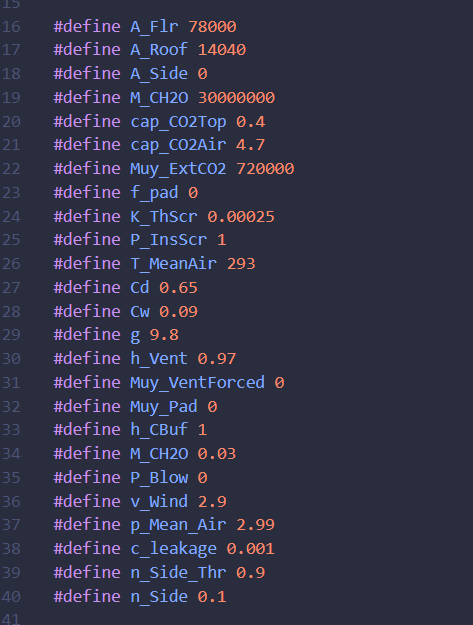
\includegraphics[width = 4in, height = 4in]{Code/Pic/constant.png}
    \caption{Declaring constants}
    \label{fig:my_label}
\end{figure}


We have a function named doublerand used to randomize the control value in the range [0,1]

\begin{figure}[h]
\centering
    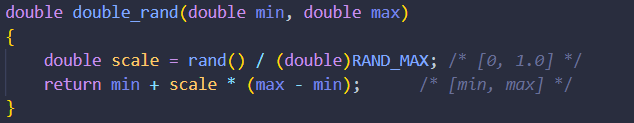
\includegraphics[width = 5.5in, height = 1.5in]{Code/Pic/random.png}
    \caption{Randomize function}
    \label{fig:my_label}
\end{figure}

The function \text{read\_record} is used to read the .csv input file

After that, we simply write the code using all the formulas mentioned in problem a of exercise 2

\begin{figure}[h]
\centering
    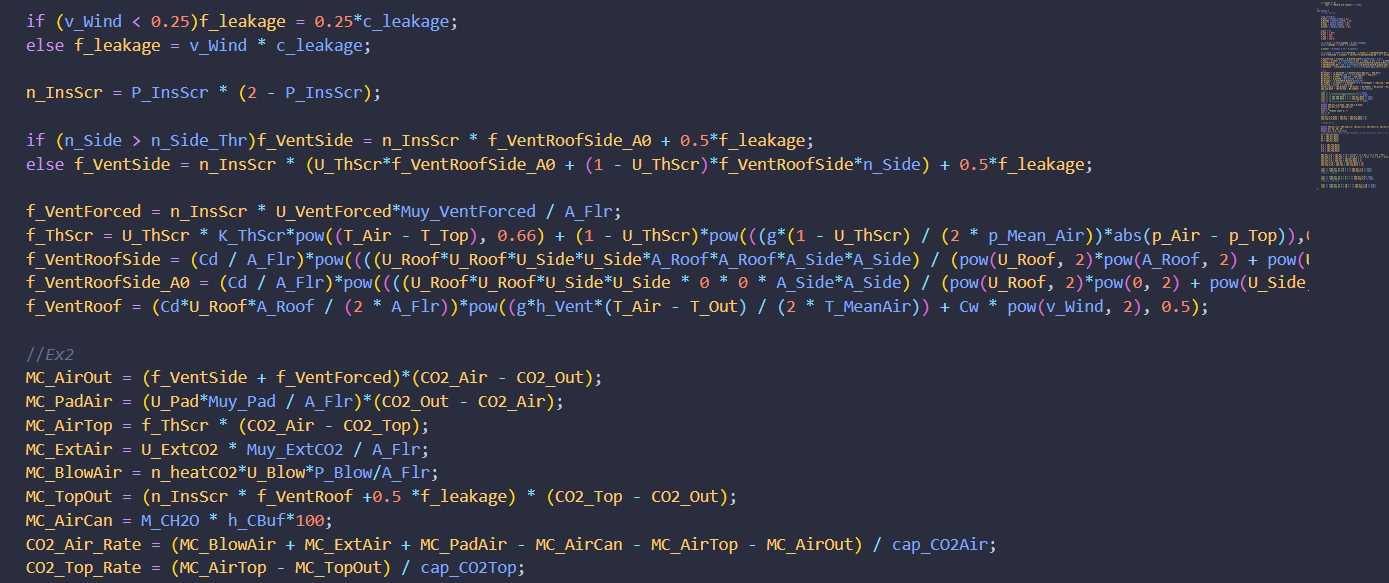
\includegraphics[width = 4in, height = 3in]{Code/Pic/ex2_code.png}
    \caption{Main code}
    \label{fig:my_label}
\end{figure}










%%%%%%%%%%%%%%%%%%%%%%%%%%%%%%%%%
\section{Exercise 3}
Ex3 give us that the temperature and density of air difference are constant so it means that $\Dot{CO2_{Air}}$ and $\Dot{CO2_{Top}}$ depend on data of CO2 concentration. However, when we did some test with data, results were almost approximately same as the first time we have done.

Follow the constant variables as the exercise 2.b above, dx and constant temperature and density of air difference as below:

\textbf{
p\_Air = 3;
p\_Top = 2.987;
T\_Air = 295;
T\_Top = 291;
T\_Out = 288.9;
}

\begin{figure}[h]
\centering
    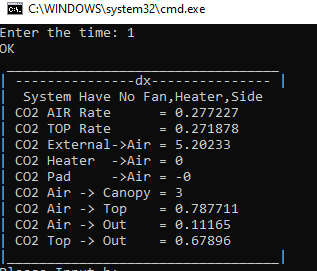
\includegraphics[width = 3in, height = 3in]{Code/Pic/result.png}
    \caption{Output}
    \label{fig:my_label}
\end{figure}

Note: There is NO Heater, NO Fan and NO sidewalls CO2 emission so that $CO2_{Heater->Air}$ and  $CO2_{Pad->Air}$ are 0 but there are still leakages on sidewalls so that $CO2_{Air->Out}$ still has a non-zero value.



\section{Exercise 4}
\subsection{Exercise 4a}
 Follow Euler Mehtod, we have:\\
\indent $CO_{2Air(thEx4a)}=CO_{2Air}+CO_{2AirRate}*h$\\
\indent $CO_{2Top(thEx4a)}=CO_{2Top}+CO_{2TopRate}*h$
 Follow order 4 Runge-Kutta method, we have:\\
\indent $k_{1}=f(tn,xn)$;\\
\indent $k_{2}=f(tn+0.5*h,xn+0.5*h*k_{2})$;\\
\indent $k_{3}=f(tn+0.5*h,xn+0.5*h*k_{2})$;\\
\indent $k_{4}=f(tn+h,xn+0.5*h*k_{3})$;\\
\indent $xn+1=xn+(\frac{1}{6})*h*(k_{1}+2k_{2}+2k_{3}+k_{4})$;\\
 However, as we tested the derivatives of $CO_{2AirTop}$ over the derivatives of time are constant so that: $k_{1}=k_{2}=k_{3}=k_{4}=CO_{2AirTopRate}$. We have:\\
\indent $CO_{2AirTop(t+h)}=CO_{2AirTop}+(\frac{1}{6})*h*(6*CO_{2AirTopRate})$\\
 Where,\\
$CO_{2Air(thEx4a)}$ is $CO_{2Air}$ at $t+h$;\\
$CO_{2Top(thEx4a)}$ is $CO_{2Top}$ at $t+h$;\\
$CO_{2AirTop(t+h)}$ is $CO_{AirTop}$ at $t+h$;\\
$CO_{2Air}$ is $CO_{2Air}$ concentration at $t$;\\
$CO_{2Top}$ is $CO_{2Top}$ concentration at $t$;\\
$CO_{2AirTop}$ is $CO_{2AirTop}$ concentration at $t$;\\
$CO_{2AirRate}$ is rate change of $CO_{2Air}$ concentration as derivative of $CO_{2Air}$ over dt;\\
$CO_{2TopRate}$ is rate change of $CO_{2Top}$ concentration as derivative of $CO_{2Top}$ over dt;\\
$CO_{2AirTopRate}$ is rate change of $CO_{2AirTop}$ concentration as derivative of $CO_{2AirTop}$ over dt;\\














\subsection{Exercise 4b}
Using Euler method in exercise 1, (figure 8)
\begin{figure}[h]
    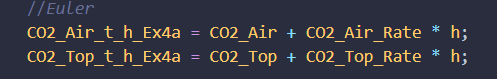
\includegraphics[width = 5.5in, height = 1in]{Code/Pic/ex4_euler.png}
    \caption{Euler Method}
    \label{fig:my_label}
\end{figure}

We already have the CO2\_Air\_Rate and CO2\_Top\_Rate in exercise 2, and h is given in this exercise, thus we already have everything we need to execute the method.

Below is the result of the programm

\begin{figure}[h]
\centering
    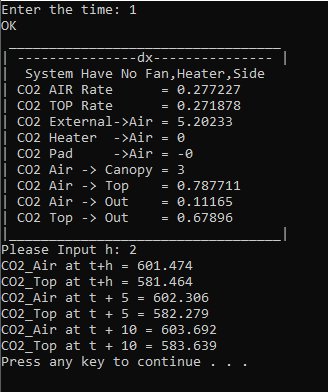
\includegraphics[width = 2.5in, height = 2.5in]{Code/Pic/final1.png}
    \caption{Programm output}
    \label{fig:my_label}
\end{figure}

\begin{figure}[h]
\centering
    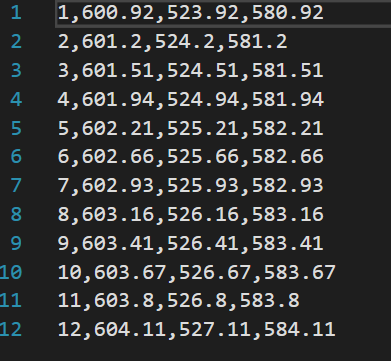
\includegraphics[width = 2in, height = 2.5in]{Code/Pic/final2.png}
    \caption{Measured data}
    \label{fig:my_label}
\end{figure}
\subsection{Conclusion}
By comparing the output with the measured data below, we can see that: 
With $t=1 \longrightarrow t+5=6, t+10=11$
\begin{itemize}
    \item CO2\_Air at 6 min is 602.306, CO2\_Top at 6 min = 582.279
    
    Compare to 
    actual data $CO_2_{Air}$ and $CO_2_{Top}$ being 602.66 and  582.66 at 6 minutes respectively
    \item CO2\_Air at 6 min is 603.692, CO2\_Top at 6 min = 583.639
    
    Compare to 
    actual data $CO_2_{Air}$ and $CO_2_{Top}$ being 603.8 and  583.8 at 6 minutes respectively
\end{itemize}

It is clear that we have a very small margin of error (around 0.02\%). Thus, the programm have a very good accuracy.














\newpage
\section{Exercise 5}
\subsection{The model for the vapor pressure}
\indent In this greenhouse climate model, the greenhouse functions heating, insulation, shading, cooling, \ch{CO2} enrichment, humidification and de-humidification are fulfilled by one or more techniques such as a direct air heater, a boiler, an industrial heat source, a geothermal source and passive buffer.\\
\indent For the improvement of a model-based plan strategy, these strategies are viewed as adequately nonexclusive for a wide scope of areas everywhere on the world. Explicit nearby answers for energy creation, energy change or atmosphere adjustment, for example,  co-generation  of  heat  and  electricity,  artificial  photosynthetic  lighting,  an  active heat buffer, a heat pump and a solar heat collector, lie outside the scope of this study. \\
\begin{center}
    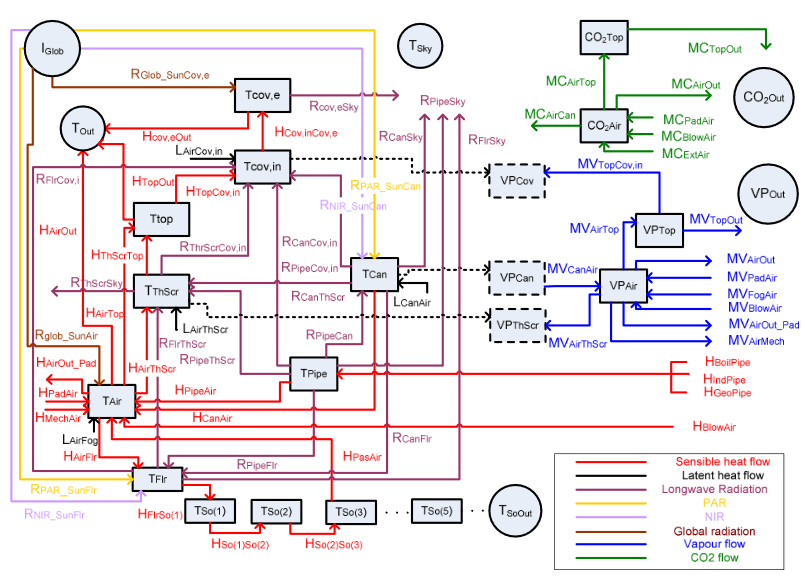
\includegraphics[width=14cm]{Image/Fi2.png}
    \captionof{figure}{\itshape{Overview of the state variables (blocks), semi-state variables (dotted blocks), external climate inputs (circles) and fluxes (arrows) of the greenhouse model. Coloured arrows represent the various energy and mass fluxes (legend at the bottom right).}}    
\end{center}
\indent Thank to De Zwart (1996), this model was based on the greenhouse climate modelling study of him. This model was added some extra elements and parts because of the current purpose.The following model elements were implemented: the design elements presented below in Figure 3. A  lumped  cover  description  to  combine  the  impact  of different  cover  layers  on  indoor  climate;  the  internal  and  external  cover  temperature  are state variables of the model to describe the impact of cover insulation on indoor climate; a description  of  the  far  infrared  radiation  (FIR)  transmission  through  the  cover,  which  is needed for films that partially transmit FIR; a description of both roof and side ventilation; a  description  of  the  impact  of  insect  screens  on  ventilation  rate;  and  a  description  of  the near  infrared  radiation  (NIR)  absorption  of  both  canopy  and  floor,  which  depend  on  the optical  properties  of  the  cover  and  floor.Since optimization of the greenhouse structure properties, i.e. greenhouse dimensions, roof slope and vent orientation and location, exceeded the purpose of our design method,
the model was simplified by not distinguishing between diffuse and direct solar radiation and by assuming that the greenhouse cover transmission coefficient was independent on solar angle.
\begin{center}
    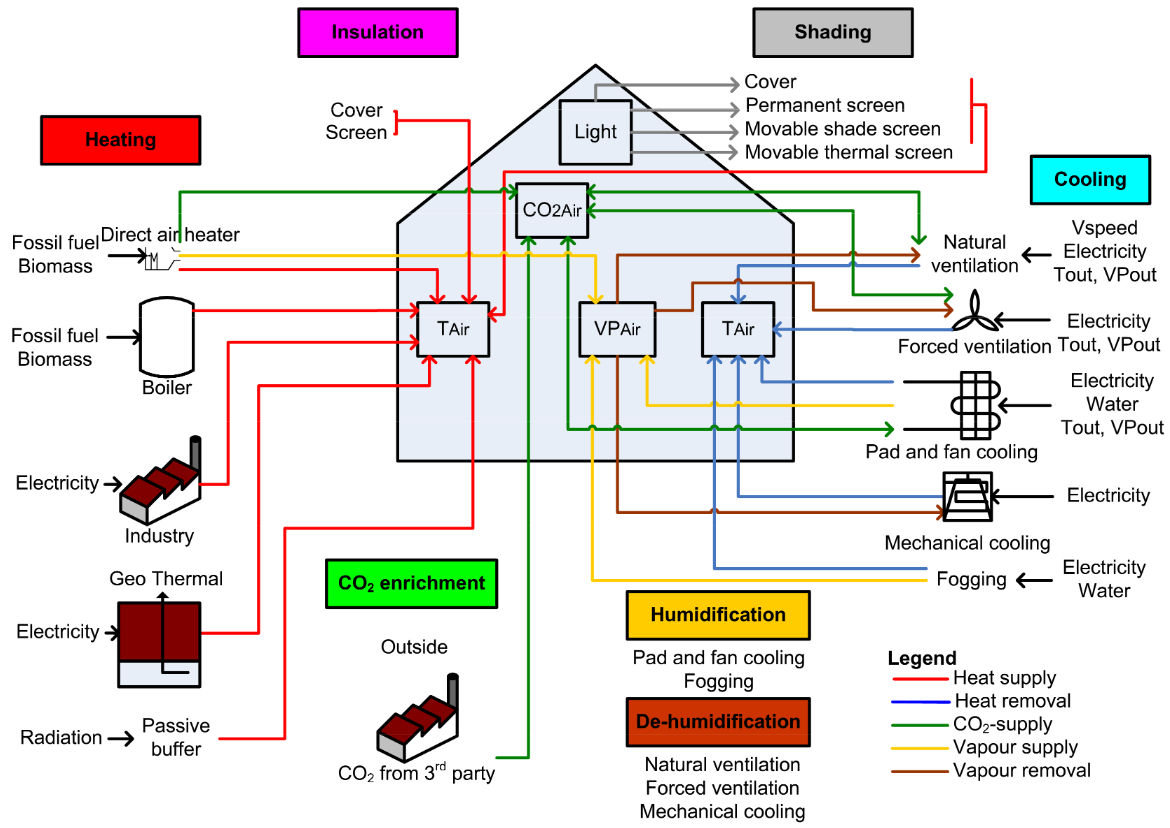
\includegraphics[width=14cm]{Image/Fi1.png}
    \captionof{figure}{\itshape{Selected functions (coloured boxes), and design elements (text blocks and pictures below the accompanying  functions),  needed  for  the  greenhouse design  method  to  manage  the  greenhouse climate (transparent boxes inside the greenhouse). The coloured arrows represent the various energy and mass fluxes (legend at the bottom right).}}    
\end{center}
\indent An overview of the states, the energy and mass fluxes of the greenhouse model is presented in Figure 2 above. This model is based on the following assumptions:
\begin{itemize}
    \item Greenhouse air is considered to be a "perfectly stirred tank" which means that no spatial differences in temperature, vapor pressure and the \ch{CO2} concentration occur. Therefore all the model fluxes are described per square metre of greenhouse floor.
    \item Describing the effect of the thermal screen on the indoor climate, the greenhouse air is divided into compartments: one below and one above the thermal screen.
\end{itemize}
\indent The conditions of the model are totally portrayed by differential conditions. The time subordinates of the states to time are introduced by a dab over the state image. All images are characterized in the Nomenclature.
\subsection{Programs calculate the net \ch{CO2} flux}
The two main equation to calculate the vapor pressure concentration in the lower and upper compartments is

\begin{equation}
\begin{array}{r}
cap_{VP_{Air}}\Dot{VP_{Air}}=MV_{CanAir}+MV_{PadAir}+MV_{FogAir}+MV_{BlowAir}-MV_{AirThScr} \\
-MV_{AirTop}-MV_{AirOut}-MV_{Airout_Pad}-MV_{AirMech}
\end{array}
\end{equation}
\begin{equation}
\begin{array}{r}
cap_{VP_{Top}}\Dot{VP_{Top}}=MV_{AirTop}-MV_{TopCov,in}-MV_{TopOut}
\end{array}
\end{equation}
However, in our model only has:
\begin{equation}
\begin{array}{r}
MV_{CanAir}=-VEC_{CanAir}(VP_{Can}-VP_{Air})
\end{array}
\end{equation}
\begin{equation}
\begin{array}{r}
VEC_{CanAir}=\frac{2\rho_{Air}c_{p.Air}LAI}{\Delta H\gamma (r_{b}+r_{s})}
\end{array}
\end{equation}

\indent Since the canopy temperature was not measured, it was assumed to be equal to the greenhouse air temperature.\\
\begin{center}
\begin{tabular}{m{7cm}m{5.5cm}m{2.5cm}}
 Density of air at sea level: & $\rho_{Air}=1.20$ & $kg m^{-3}$ \\ 
 Specific heat capacity of the air: & $c_{p.Air}=1*10^{-3}$ & $JK^{-1}kg^{-1}$ \\  
 Latent heat of evaporation: & $\Delta H=2.45*10^{6}$ & $Jkg^{-1}water$\\    
 Stefan BoltzMann constant: & $\sigma=5.670*10{-8}$ & $Wm^{-2}K^{-4}$\\    
 Psychrometric constant: & $\gamma=65.8$ & $PaK^{-1}$\\    
 Boundary layer resistance of the canopy for vapor transport: & $r_{b}=275$ & $sm^{-1}$\\
 Stomatal resistance of the canopy: & $r_{s}=r_{s.min}.rf(R_{Can}).$ & \\
  & $rf(CO_{2Air_ppm}.rf(VP_{Can}-VP_{Air})$ &$sm^{-1}$\\
 The minimum canopy resistance for transpiration : & $r_{s.min}=82.0$ & $sm^{-1}$\\  
\end{tabular}
\end{center}
 \indent \indent \indent \indent \indent \indent \indent \indent$rf(R_{Can})=\frac{R_{Can}+c_{evap1}}{R_{Can}+c_{evap2}}$ \\
 \indent \indent \indent \indent \indent \indent \indent$rf(CO_{2Air}=1+c_{evap3}(\eta_{mg_{ppm}CO_{2Air}-200)^{2}}$ \\
 \indent \indent \indent \indent \indent \indent \indent$rf(VP_{Can}-VP{Air}=1+c_{evap4}(VP_{Can}-VP_{Air})^{2}$ \\
\begin{center}
\begin{tabular}{m{7.5cm}m{3cm}m{2.5cm}}
Coefficient of the stomatal resistance model to account for radiation effect&$c_{evap1}=4.30$& $Wm^{-2}$\\
Coefficient of the stomatal resistance model to account for radiation effect&$c_{evap2}=0.54$& $Wm^{-2}$\\
Coefficient of the stomatal resistance model to account $CO_{2}$ effect&$c_{evap3}^{day}=6.1*10{-7}$   $c_{evap3}^{night}=1.1*10{-11}$& $ppm^{-2}$\\
Coefficient of the stomatal resistance model to account for vapor pressure difference&$c_{evap4}^{day}=4.3*10{-6}$ $c_{evap4}^{night}=5.2*10{-6}$& $Pa^{-2}$\\

\end{tabular}
\end{center}
\indent The general form of a vapour flux accompanying an air flux is described by:
\newline
$MV_{12}=\frac{M_{Water}}{R}f_{12}(\frac{VP_{1}}{T_{1}+273.15}-\frac{VP_{2}}{T2+273.15}$ \indent $kgm^{-2}s^{-1}$\\
\indent where $MV_{12}$ is the vapor flux from location 1 to location 2, $f_{12}(m^{3}m^{-2}s^{-1})$ is the air flux from location 1 to location 2, $T_{1}$($^{o}{C}$) is the temperture at location 1 and $T_{2}$($^{o}{C}$) is the temperature at location 2.
\indent The vapor fluxes $MV_{AirTop}$, and $MV_{TopOut}$ are described above analogously. Where by their accompanying air fluxes are $f_{ThScr}$ (the flux through the thermal screen), $f_{VentRoof}$ (flux due to roof ventilation) respectively. We have $VP_{Top}$ and $VP_{Air}$ as input, while $VP_{Out}=1.0$\\
$f_{ThScr}=U_{ThScr}K_{ThScr}|T_{Air}-T_{Out}|^{0.66}+\frac{1-U_{ThScr}}{\rho_{Air}^{Mean}}(0.5\rho_{Air}^{Mean}(1-U_{ThScr})g|\rho_{Air}-\rho_{Out}|)^{0.5}$\\
$K_{ThScr}=0.0002$5\indent $\rho_{Air}^{Mean}=2.99$ \indent \indent $m^{3}m^{-2}s^{-1}$\\
\indent The density of the air is elevation dependent and by assuming a mean air temperature of $20^{o}C$ the density of the air is calculated by:\\
$\rho_{Air}=\rho_{Air0}exp(\frac{gM_{Air}h_{Elevation}}{293.15R})$ \indent \indent $kgm^{-3}$\\
\indent Density of air at sea level $\rho_{Air0}=1.20kgm^{-3}$ and $h_{Elevation}=1470(m)$\\
\indent Molar mass of air: $M_{Air}=28.96 kgkmol^{-1}$\\
\indent $R (Jkmol^{-1}K^{-1})$ is the molar gas constant $g=9.81$
\begin{equation}
f_{\text {VentRoof}}=\left\{\begin{array}{l}
\eta_{\text {Ins}Scr} f_{\text {VentRoof}}^{\prime \prime}+0.5 f_{\text {leakage}}\indent \indent \indent \indent \indent \indent \indentif\eta{roof} \geq \eta_{Roof_Thr}\\
\eta_{\text {Ins}Scr}\left[U_{\text {ThScr}} f_{\text {VentRoof}}^{\prime \prime}\right. \\
\left.+\left(1-U_{\text {ThScr}}\right) f_{VentRoofSide}^{\prime \prime} \eta_{\text {Side }}\right]+0.5 f_{\text {leakage}}\indent if \eta_{Roof}<\eta_{Side_Thr} \\
\indent \indent \indent \indent \indent \indent\indent \indent \indent \indent \indent \indent\indent \indent \indent \indent m^{3}m^{-2}s^{-1}
\end{array}\right.
\end{equation}
\indent The natural ventilation  rate due to roof ventilation is described by Boulard and Baille (1995):
$f_{VentRoof}^{\prime \prime} = \frac{U_{Roof}A_{Roof}C_{d}}{2A_{Flr}}\sqrt{\frac{gh_{Vent}}{2}\frac{T_{Air}-T_{Out}}{T+273.15}+C_{w}v_{Wind}^{2}}$ \indent $m^{3}m^{-2}s^{-1}$\\
\indent $\eta_{Roof_Thr}=0.9$ is the ration between the roof vent area and total ventilation are above no chimney effect and was assumed.
\indent Our model $\eta_{Roof}=1$ since we only have top roof vent, and no insect screen to reduce ventilation rate: $f_{VentRoof}=f_{VentRoof}^{\prime \prime}+0.5f_{leakage}$\\
\indent Furthermore the ventilation rate of the greenhouse is influenced by the greenhouse leakage rate which depends on wind speed and is described by:\\
\begin{equation}
f_{\text {leakage}}=\left\{\begin{array}{l}
0.25*c_{leakage}, \indent v_wind < 0.25 \indent \indent m^{3}m^{-2}s^{-1}\\
c_{leakage*v_{wind}}, \indent v_{wind} \geq 0.25
\end{array}\right.
\end{equation}
\indent Because our $v_{wind}=0.29$ so we $2nd$ formula: $c_{leakage}*v_{wind}$, where $c{leakage}=1*10^{-4}$\\
\indent To calculate $A_{Roof}$, we multiply the specific roof ventilation area $A_{Roof}/A_{Flr}=0.18$ to the surface of the greenhouse floor $A_{Flr}=7,8*10^{4} m^{2}$, which result is $14040 (m^{2})$.\\
\indent $C_{d}=C_{d}^{Gh}(1-\eta_{ShScrC_{d}}U_{ShSc})$\\
\indent$C_{w}=C_{w}^{Gh}(1-\eta_{ShScrC_{w}}U_{ShSc})$\\
\indent Where $C_{d}^{Gh}=0.65$ and$C_{w}^{Gh}=0.9$ for Texas model, since we do not have moving shading screen so the parameter that determines the effect of the movable shading screen on the discharge coefficient $\eta_{ShScrC_{d}} = 0$ and ${ShScrC_{w}}=0$. Other needed variables is: $h_{vent}= 0.97$, $T_{Out}= 23.9 C$, $VP_{out}=1.3$, $T_{Air}=6.8$, $VP_{Air}=12.8$.\\

\begin{thebibliography}{80}


\bibitem{bib1}
Bram HE Vanthoor.
\textit{A model-based greenhouse design method.}
2011

\bibitem{bib2}
Vanthoor, C. Stanghellini,  E.J. van Henten and P.H.B. de Visser.
\textit{A methodology for model-based greenhouse design}

\bibitem{bib3}
David Katzin, Simon van Mourik, Frank Kempkes, Eldert J. van Henten
\textit{
GreenLight - An open source model for
greenhouses with supplemental lighting:
Evaluation of heat requirements under LED
and HPS lamps}


\end{thebibliography}
\end{document}

